\documentclass{report}
\usepackage{amsmath}
\usepackage{amsfonts}
\usepackage{pifont}
\usepackage{color}
\usepackage{graphics, epstopdf}
\usepackage[pdftex]{graphicx}
\usepackage[pdftex]{hyperref}
\usepackage{verbatim}
\usepackage{amsthm}
\usepackage{cleveref}
\usepackage{caption}
\usepackage{subcaption}
\urlstyle{same}

\newcommand{\com}[1]{
	\vspace{0.2cm}
	\noindent
	\emph{#1}
}

\definecolor{gray}{gray}{0.5}
\hypersetup{colorlinks, citecolor=black, filecolor=black, linkcolor=black, urlcolor=gray}

\newcommand{\code}[1]{\texttt{#1}}

\newtheorem{mydef}{Definition}
    
\begin{document}

\title{Image classification with deformations}

\author{Gustav Larsson}

\maketitle

%\begin{abstract}
%
%Using wavelet deformations of mixture component templates, to 
%Classifying well-posed handwritten digits (MNIST) using binary edge features and wavelet-based deformations. 
%
%\keywords{score following, real-time score alignment, automatic accompaniment}
%\end{abstract}
%
\chapter{Edge features}

\section{Introduction}
MNIST is a dataset of well-posed (centered) and clean (little noise) digits of 10 classes. The task is to determine which class an image belongs to, by training several prototypes of each class and comparing an image to the prototypes. The image is converted to binary features, which are assumed to be drawn independently from Bernoulli distributions (the prototype).
The prototypes are also allowed to deform using a wavelet basis to match the image better, to the cost of a Gaussian prior over the parameters of the deformation.

\section{Method}

% ----------------------------------------------------------------------------------
%The input data consists of gray-level intensities. Each pixel is converted to 8 binary directed edge features according to ch.~5.4 in Amit's book. Each feature represents the presence of an edge in one of $J$ directions.
%In order to get robust edges, I use $k=5$ and pixel inflation (each actual edge, will result in its 8 closest neighbors becoming edges too). 
%Each original image, before feature extraction, is $28 \times 28$ with intensities in $[0, 1]$. The image is padded with zeros to $32 \times 32$ to play nicer with the wavelet transforms. 
 %4 for the cardinal and 4 for the di %1 indicating an edge, and 0 not. 

\subsection{Definitions} \label{sec:defs}

This document largely follows the same notation as in Yali Amit's book (Chapter~5). Here is a condensed form: 

\begin{mydef}
Let $Y$ be the set of all classes; $K$ the set of all coefficient indices for a wavelet transform; $Q = \{1,2\}$ the two axes in an image; $J$ the set of all directed edge features for each pixel.% TODO move: We use $|J| = 8$, representing directed edges in the 4 cardinal and the 4 diagonal directions.
\end{mydef}

\begin{mydef}
$L \in Z^{d}$ is a fixed image grid of $d$ points $z \in Z = \mathbb{R}^2$, making up the pixel locations of an undeformed image. %, making up the pixel locations of an undeformed image with $d$ pixels. 
\end{mydef}

\begin{mydef}
Let the family of images, converted to edge features, be $\mathcal{X} = \{ (X_1, \dots, X_{|J|}) \mid X_j : L \rightarrow \{0,1\}\}$, where the function value represents the presence of an edge.% We shall also allow $I(x)$ to evaluate
\end{mydef}

\begin{mydef}
Let the family of prototypes be $\mathcal{F} = \{ (F_1, \dots, F_{|J|}) \mid F_j : Z \rightarrow [0, 1]\}$, where the function value represents a Bernoulli probability. Notice that the functions are defined on the entire space $Z$, and not just the image grid $L$.
\end{mydef}

%For $\mathcal{F}$ and gradients thereof, we shall allow the mappings to take an argument $x \in Z \not\subset L$ (outside the pixel lattice), and assume it to be a bilinear interpolation of surrounding values. If $x$ is outside the grid, we shall take the closest edge value for functions, and 0 for all partial derivatives.

\subsection{Data model}
Now, assume that each edge feature in the image $X \in \mathcal{X}$ was generated from a deformed prototype image $F \in \mathcal{F}$. The deformation is parameterized by $u$ as

\[
    U(x) = (\Psi^{-1}(u^{(1)}), \Psi^{-1}(u^{(2)})),
\]
where $\Psi$ denotes a wavelet transform, and $u^{(q)}$ all necessary coefficients for axis $q$. We have
\[
    \Psi^{-1}(u) = \sum_{k\in K} u_k \psi_k(x),
\]
where $\psi_k$ is the wavelet basis functions associated with $k \in K$ the set of coefficients.

Now, the deformation and the image are assumed to be drawn from the following distributions:

\begin{align}
    u^{(q)}_{k} &\sim \mathcal{N}(\mu^{(q)}_{k}, (\lambda^{(q)}_{k})^{-1}), &q \in Q, k \in K, \label{eq:gaussian} \\
    X_j(x) &\sim \text{Bern}(F_j(\tilde x)), &x \in L, j \in J, \label{eq:bernoulli}
 \end{align}
where we introduce the short-hand $\tilde x = x + U(x)$.

The parameters $\mu$ and $\lambda$ are specific to the prototype $F$.
Notice that we then have
\begin{equation} \label{eq:partial_tilde}
    \frac{\partial \tilde x^{(q)}}{\partial u_k} = \psi_k.
\end{equation}

We now set a cost function to the negative posterior, ignoring any additive constants, and get (not be confused with the set $J$)

\begin{align*}
    J(u) =& \frac{1}{2} \sum_{q\in Q} \sum_{k\in K} \lambda^{(q)}_k (u^{(q)}_k -\mu^{(q)}_k)^2 - \\
        &\sum_{j\in J} \sum_{x \in L}  \left( 
            X_j(x) \log(F_j(\tilde x))   +   (1-X_j(x)) \log(1-F_j(\tilde x)) \right)
\end{align*}
Taking partial derivatives of this we get
\begin{align*}
    \frac{\partial J(u)}{\partial u^{(q)}_k} =& \lambda^{(q)}_k (u^{(q)}_k -\mu^{(q)}_k) - \\    
    & \sum_{j\in J} \sum_{x \in L} 
        \left( \frac{X_j(x)}{F_j(\tilde x)} - \frac{1-X_j(x)}{1-F_j(\tilde x)} \right) 
                \partial_q F_j(\tilde x) \psi_k(x),
\end{align*} 
where $\partial_q$ indicates the partial derivative along the $q$ axis.

\subsection{Minimization}

We define the best deformation as
\[
    \hat u = \arg\min_u J(u).
\]
This is determined using a Quasi-Newton search algorithm (specifically BFGS), which uses repeated evaluations of $J(u)$ and $\nabla J(u)$ to find the minimum. The process is done in a coarse-to-fine manner, by initially using $S_0$ coefficient levels, letting them converge, and then increase the number of levels to and including $S$.

The minimum cost $J(\hat u)$ now gives us a value that we can compare between prototypes $F$, to determine the most likely one. 

%\section{Classification}
%Given a set of classes $

\subsection{Classification}

We shall denote the parameters of a prototype as $\theta = (F, \mu, \lambda, y)$, where $y \in Y$, denotes the class that the prototype is representing. Let $\Theta$ denote the set of all such parameter tuples, and allow multiple entries with the same class $y$.

It is appropriate to now write $J_{\theta}(u)$ as the cost function associated with $\theta$ and the image $X$.

Classification, i.e. determining the class of $X$, denoted $\hat y$, is done by taking
\[
    \hat \theta = \arg\min_{\theta \in \Theta} J_{\theta}(\hat u),
\]
which of course contains $\hat y$.


%We shall denote the selection of all parameters as $\Theta$, and it will encompass $T$ prototypes 

\subsection{Learning}

Building $\Theta$ is done by taking $N$ images of each class and running a Bernoulli mixture model for each with $M$ components. The templates of the mixture model constitutes the prototypes $F$. For stability, allow only $F_j(x) \in [\delta, 1-\delta]$, for some small value $\delta > 0$. 

The domain of the functions $F_j$ is extended to the entire $Z$ by bilinear interpolation. Values outside the grid are given the closest edge value in $F_j$.

The gradient $\nabla F_j$ is calculated by central differences with sample distance 1 in the middle and the first difference on the boundaries. Values outside $L$ are evaluated again by bilinear interpolation, however this time the fill value outside the grid is 0.

The parameters of the prior, $\mu$ and $\lambda$, are learned as follows. Each template is associated with a set of original training images (mixture component affinities are assumed to be degenerate for all images, meaning each image has contributed to only one mixture component). For each image, $\hat u$ is determined by the method above, using a predetermined and fixed $\mu_0$ and $\lambda_0$. The values $\mu$ and $\lambda$ associated with this template is now extracted as the mean and precision (inverse variance) of those $\hat u$ values.

The values $\mu_0$ are set to $\mathbf{0}$, since the template is expected to match well with the identity deformation. The values $\lambda_0$ are set as following for both axes (omitting $(q)$ from the notation)
\[
    \lambda_{k} = \lambda_{(\alpha, s, l_1, l_2)} = \eta 2^{\rho s}
\]
where $\eta$ is a fairly arbitrarily scaled penalty term and $\rho > 0$ is a smoothening term. The coefficient index $k$ breaks up to $\alpha \in \{HG, GH, HH\}$, the dilations $0 \le s \le S$ and the translations $0 \le l_1, l_2 < 2^s$. The value $s = 0$ represents the scaling function (as opposed to the wavelet functions) and thus has only one $\alpha$ value. The value $S$ dictates how many levels of wavelet functions to use, which is determined beforehand. This means that setting $S=0$, only the scaling function is used.

%The model can also be run by using $\mu_0$ and $\lambda_0$ directly.

%For each class, $N$ images per class are used to train a Bernoulli mixture model of $K$ components (so far, fixed and manually determined). This means that 

\subsection{Experiments}
Classification can be done without deformation, using only the mixture model (NoDeform) or with deformations (Deform). As a speed optimization, you can also employ deformation only if there are other prototypes within a factor $\alpha$ of the minimum cost without deformations, in which case all those become contendors and are deformed (SelDeform).

The MNIST dataset consists of images of size $28 \times 28$ with gray-level intensities. The images are zero-padded to $32 \times 32$ to work better with the wavelet transform. Each pixel is then converted to 8 binary features. The directed edge features are described in Yali Amit's book (Chapter 5.4) and we use $k=5$ with feature inflation (the 8 neighbors of an edge are also reported as edges).

\subsection{Conjugate prior}
% surplus1.npz:  python run_classifier.py -d edges -a 1.2 --test-conjugate 0 0.0001 100.0 200 -l 100 --rho 1 -s surplus1.npz c/eval-feat.npz c/mixtures.npz c/coefs.npz  
% surplus2.npz:  python run_classifier.py -d edges -a 1.2 --test-conjugate 0 0.0001 100.0 200 -l 10 --rho 2.7 -s surplus2.npz c/eval-feat.npz c/mixtures.npz c/coefs.npz  
% surplus3.npz:  python run_classifier.py -d edges -a 1.2 --test-conjugate 0 0.01 100.0 200 -l 10 --rho 2.7 -s surplus3.npz c/eval-feat.npz c/mixtures.npz c/coefs.npz  
% surplus4.npz:  python run_classifier.py -d edges -a 1.2 --test-conjugate 0 0.1 10.0 2000 -l 10 --rho 2.7 -s surplus4.npz c/eval-feat.npz c/mixtures.npz c/coefs.npz  
% surplus5.npz:  python run_classifier.py -d edges -a 1.2 --test-conjugate 0 0.1 100.0 2000 -l 100 --rho 1.0 -s surplus5.npz c/eval-feat.npz c/mixtures.npz c/coefs.npz  
% surplus6.npz:  python run_classifier.py -d edges -a 1.2 --test-conjugate 0 1.0 100.0 200 -l 100 --rho 1.0 -s surplus6.npz c/eval-feat.npz c/mixtures.npz c/coefs.npz  
% surplus7.npz:  python run_classifier.py -d edges -a 1.2 --test-conjugate 0 1.0 10.0 200 -l 10 --rho 2.7 -s surplus7.npz c/eval-feat.npz c/mixtures.npz c/coefs.npz  


% itercoefs1.npz: python train_def_coefs.py -l 100 --rho 1 -n 12 -b 0.05 c/training-feat.npz c/mixtures.npz c/itercoefs1.npz
% itercoefs2.npz: python train_def_coefs.py -l 10 --rho 2.7 -n 12 -b 0.05 c/training-feat.npz c/mixtures.npz c/itercoefs2.npz
% itercoefs3.npz: python train_def_coefs.py -l 100 --rho 1 -n 12 -b 0.2 c/training-feat.npz c/mixtures.npz c/itercoefs3.npz
% itercoefs4.npz: python train_def_coefs.py -l 10 --rho 2.7 -n 12 -b 0.2 c/training-feat.npz c/mixtures.npz c/itercoefs4.npz
% itercoefs5.npz: python train_def_coefs.py -l 100 --rho 1 -n 12 c/training-feat.npz c/mixtures.npz c/itercoefs5.npz
% itercoefs6.npz: python train_def_coefs.py -l 10 --rho 2.7 -n 12 c/training-feat.npz c/mixtures.npz c/itercoefs6.npz
% itercoefs7.npz: python train_def_coefs.py -l 100 --rho 1 -b 0.0001 -n 12 c/training-feat.npz c/mixtures.npz c/itercoefs7.npz
% itercoefs8.npz: python train_def_coefs.py -l 10 --rho 2.7 -b 0.0001 -n 12 c/training-feat.npz c/mixtures.npz c/itercoefs8.npz

% itercoefs9.npz: python train_def_coefs.py -l 100 --rho 1.0 -n 12 -b 0.005 c/training-feat.npz c/mixtures.npz c/itercoefs9.npz
% itercoefs10.npz: python train_def_coefs.py -l 100 --rho 1.0 -n 12 -b 0.0005 c/training-feat.npz c/mixtures.npz c/itercoefs10.npz
% itercoefs11.npz: python train_def_coefs.py -l 100 --rho 1.0 -n 12 -b 0.5 c/training-feat.npz c/mixtures.npz c/itercoefs11.npz

% Testing different iterative trainings (through classification, not surplus)
% python run_classifier.py -d edges -a 1.4 c/testing-feat.npz c/mixtures.npz c/itercoefs10.npz
\begin{comment}
Deformed: 67.40%
Average contendors: 11.55
Incorrect and undeformed: 0.00%
Turned correct, incorrect: 5.80%, 1.00%
Miss rate: 2.70% (27/1000)
\end{comment}

% python run_classifier.py -d edges -a 1.4 c/testing-feat.npz c/mixtures.npz c/itercoefs9.npz
\begin{comment}
Deformed: 67.40%
Average contendors: 11.55
Incorrect and undeformed: 0.00%
Turned correct, incorrect: 5.90%, 1.00%
Miss rate: 2.60% (26/1000)
\end{comment}

% python run_classifier.py -d edges -a 1.4 c/testing-feat.npz c/mixtures.npz c/itercoefs1.npz
\begin{comment}
Deformed: 67.40%
Average contendors: 11.55
Incorrect and undeformed: 0.00%
Turned correct, incorrect: 5.60%, 1.10%
Miss rate: 3.00% (30/1000)
\end{comment}

% python run_classifier.py -d edges -a 1.4 c/testing-feat.npz c/mixtures.npz c/itercoefs11.npz
\begin{comment}
Deformed: 67.40%
Average contendors: 11.55
Incorrect and undeformed: 0.00%
Turned correct, incorrect: 4.80%, 1.10%
Miss rate: 3.80% (38/1000)
\end{comment}


%%%%%%%%% Tests with entire dataset
% python run_classifier.py -d edges -a 1.4 c/all-testing-feat.npz c/mixtures.npz c/itercoefs10.npz
\begin{comment}
Deformed: 71.06%
Average contendors: 12.47
Incorrect and undeformed: 0.01%
Turned correct, incorrect: 6.96%, 1.10%
Miss rate: 3.28% (328/9999)
\end{comment}

% python run_classifier.py -d edges -a 1.4 c/all-testing-feat.npz c/mixtures.npz c/itercoefs9.npz
\begin{comment}
Deformed: 71.06%
Average contendors: 12.47
Incorrect and undeformed: 0.01%
Turned correct, incorrect: 6.97%, 1.19%
Miss rate: 3.36% (336/9999)
\end{comment}

% python run_classifier.py -d edges -a 1.4 c/all-testing-feat.npz c/mixtures.npz c/itercoefs1.npz
\begin{comment}
Deformed: 71.06%
Average contendors: 12.47
Incorrect and undeformed: 0.01%
Turned correct, incorrect: 6.76%, 0.93%
Miss rate: 3.31% (331/9999)
\end{comment}

% python run_classifier.py -d edges -a 1.4 c/all-testing-feat.npz c/mixtures.npz c/itercoefs11.npz
\begin{comment}
Deformed: 71.06%
Average contendors: 12.47
Incorrect and undeformed: 0.01%
Turned correct, incorrect: 6.01%, 0.95%
Miss rate: 4.08% (408/9999)
\end{comment}


Learning $\lambda$ values runs the risk of overfitting or getting the wrong scale since the likelihood term is underrated (because pixels are falsely assumed to be independent). In this section we investigate the effects of putting a Gamma prior over $\lambda$ in the Gaussian distribution in (\ref{eq:gaussian}). Since we have several values of $\lambda$, we will actually have a Gamma prior over each of those values, according to the following density function
\[
    \text{Gam}(\lambda|a,b) = \frac{b^{a}}{\Gamma(a)}\lambda^{a-1}e^{-b x},
\]
with
\[
    \text{E}[\lambda] = \frac{a}{b}, \text{Var}[\lambda] = \frac{a}{b^2}.
\]

Instead of controlling the hyperparameters $a$ and $b$, we will decide a reasonable value for what the most probable value of $\lambda$ should be, and then adjust the variance by setting $b$. The relationship is given by deriving the Gamma distribution with regards to $\lambda$, setting the expression to zero. This gives
\begin{equation} \label{eq:gammamax}
    \arg\max_{\lambda} \text{Gam}(\lambda|a, b) = \frac{a-1}{b}.
\end{equation}
We want to set $\lambda$ through $\eta$ and $\rho$ as described earlier, and then adjust $b$ as needed, this gives us
\[
    a = b \eta 2^{\rho s} + 1
\]
Omitting some calculations, this gives us expressions of $a_N$ and $b_N$ for the posterior distribution. From that we extract $\lambda_N$, the maximum of our posterior distribution according to (\ref{eq:gammamax}) as
\[
    \lambda_N = \frac{b_0 \lambda_0 + \frac{N}{2}}{b_0 + \frac{N}{2 \lambda_{ML}}},
\]
where $\lambda_{ML} = \sigma_{ML}^{-2}$ is the sample precision and $N$ the sample size.

\newcommand{\FT}{F$_\rightarrow $T}
\newcommand{\TF}{T$_\rightarrow $F}

\section{Preliminary results}
All experiments here are on subsets of the MNIST dataset, so the number of classes is $|Y| = 10$. The number of training samples is given by $N \cdot |Y|$. The tables contain the following information:
\begin{itemize}
    \item[\textbf{\FT}] Denote how many classifications that were False with the mixture model alone, but turned True as a result of deformations.
    \item[\textbf{\TF}] Analogous to \FT.
    \item[\textbf{Deformed}] Percentage of test cases that employed deformations. 
    \item[\textbf{\#cont.}] Average number of deformations made for all cases where deformations were employed.
    \item[\textbf{F undef.}] Percentage of test cases that were classified F and did not use deformations (meaning, $\alpha$ might be too small if this is greater than zero).
\end{itemize}

\subsection{Preliminary results 1 and influence of $\alpha$}
Setting $N=100, M=5, \eta=100, \rho=1, S_0=1, S=3, \delta=0.05$ and using Daubechies D8 wavelets for $\Psi$. This trial was tested on 1000 samples from the training set (disjoint from the subset used for training). We tried several values of $\alpha$. Results in tab.~\ref{tab:trial1}.

\begin{table}
    \begin{center}
        \begin{tabular}{ | l | l | l | l | l | l | l | l | }
            \hline
            Method & $\alpha$ & Miss rate & \FT & \TF & Deformed & \#cont. & F undef. \\
            \hline
            NoDeform  & 1.0               & 7.50\% & - & - & - & - & - \\ 
            SelDeform & 1.1 & 4.80\% & 3.40\% & 0.70\% & 17.90\% & 3.70 & 1.90\% \\
            SelDeform & 1.2 & 3.90\% & 4.70\% & 1.10\% & 35.90\% & 5.60 & 0.40\% \\
            SelDeform & 1.3 & 3.00\% & 5.50\% & 1.00\% & 52.20\% & 8.22 & 0.10\% \\
            SelDeform & 1.4 & 2.90\% & 5.60\% & 1.00\% & 67.40\% & 11.55 & 0.00\% \\
            SelDeform & 1.5 & 2.90\% & 5.60\% & 1.00\% & 78.00\% & 15.58 & 0.00\% \\
            Deform    & $\infty$  & 2.90\% & 5.60\% & 1.00\% & 100.00\% & 50.00 & 0.00\% \\
            \hline
        \end{tabular}
    \end{center}
    \caption{Shows improvement of deformations and influence of $\alpha$.} \label{tab:trial1}
\end{table}

\subsection{Conjugate prior}
Tried $\eta=100, \rho=1$, which was used in Trial 1 above. Also tried $\eta=10, \rho=2.7$, which was very roughly chosen to be somewhat similar to the trained shape of the different coefficient levels, just to see how it would affect the results. Results can be seen in \cref{fig:b0,fig:b0zoom,fig:rho1,fig:rho27}.

Since this a search space in $\eta$, $\rho$ and $b_0$, this is a very shallow investigation so far.

\begin{figure}
    \centering
    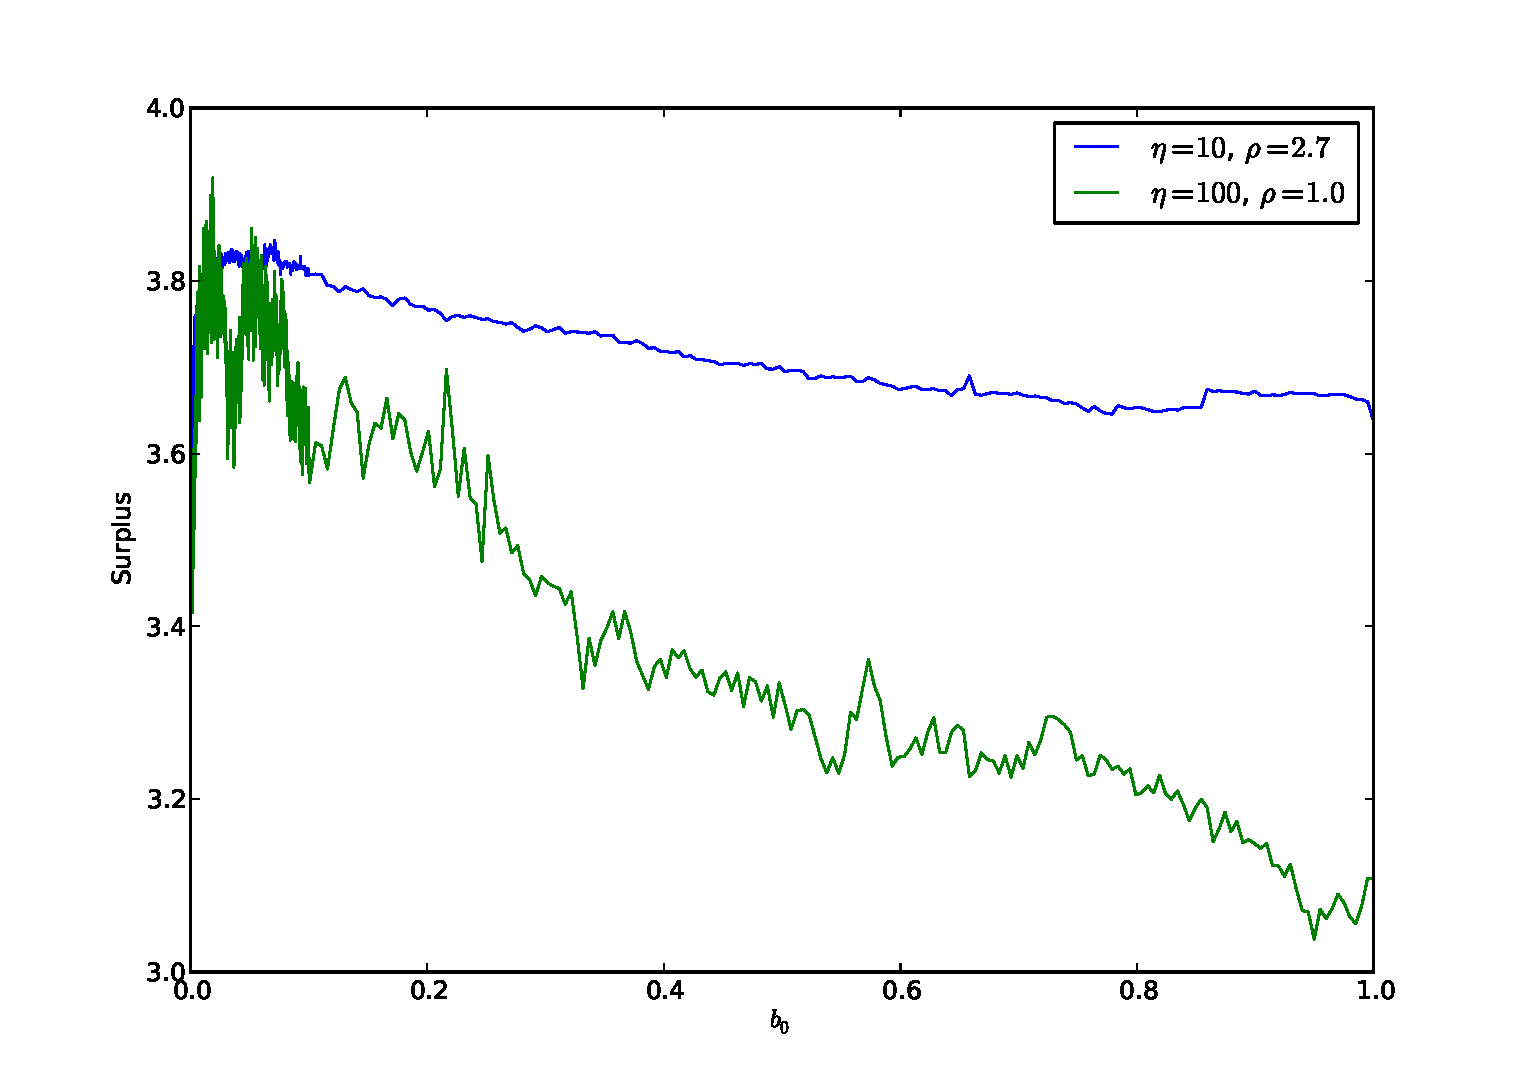
\includegraphics[width=0.8\textwidth]{figs/surplus45b.pdf}
    \caption{Two different values of $\eta$ and $\rho$ are tried. The granularity of $b_0$ changes after 0.1 to save some calculation time.} \label{fig:b0}
\end{figure}

\begin{figure}
    \centering
    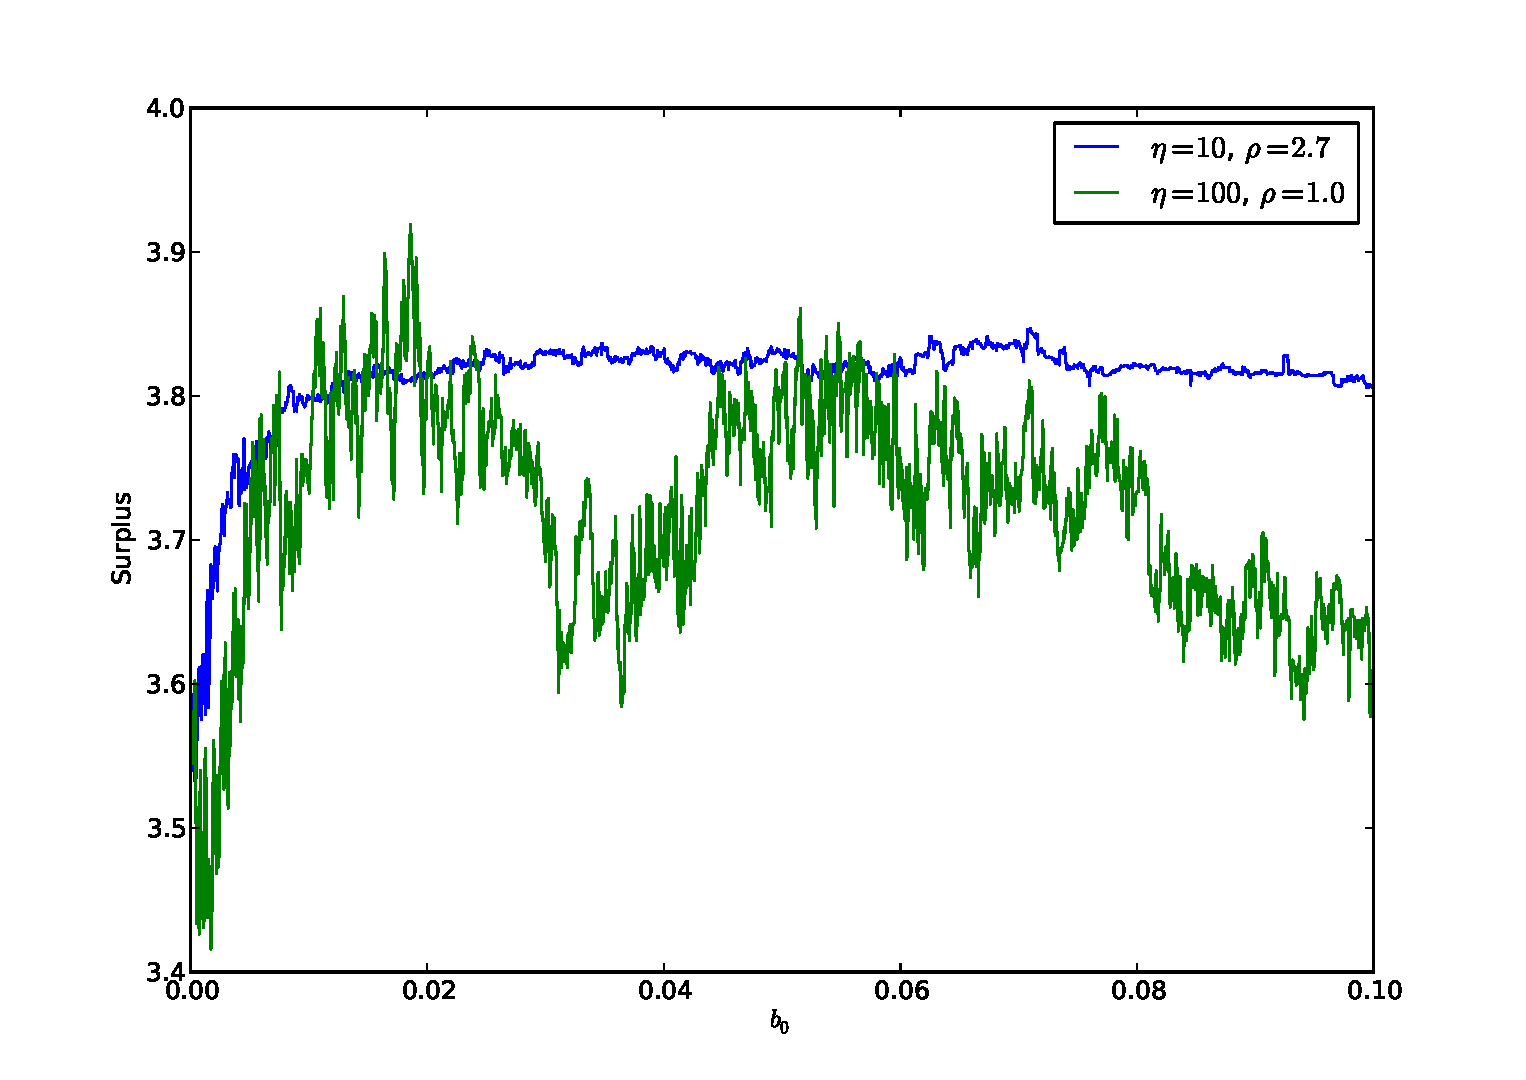
\includegraphics[width=0.8\textwidth]{figs/surplus45.pdf}
    \caption{Same as fig.~\ref{fig:b0}, except zoomed in.} \label{fig:b0zoom}
\end{figure}


\begin{figure}
    \centering
    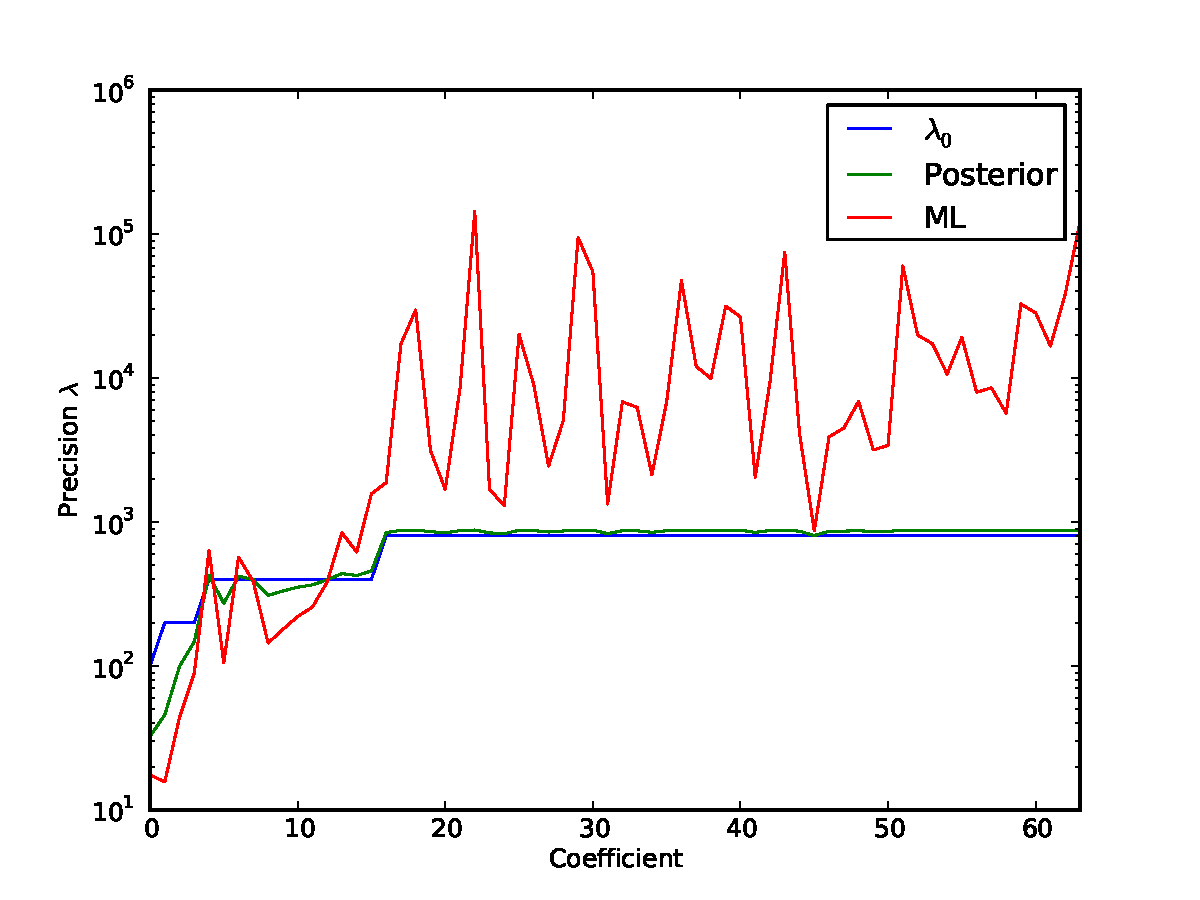
\includegraphics[width=0.8\textwidth]{figs/plotb000-eta100-rho1.pdf}
    \caption{Prior ($\lambda_0$), likelihood (ML) and posterior of the coefficients for $\eta=100$ and $\rho=1$ at $b_0 = 0.05$. For digit 0, mixture component 0 and axis 0.} \label{fig:rho1}
\end{figure}

\begin{figure}
    \centering
    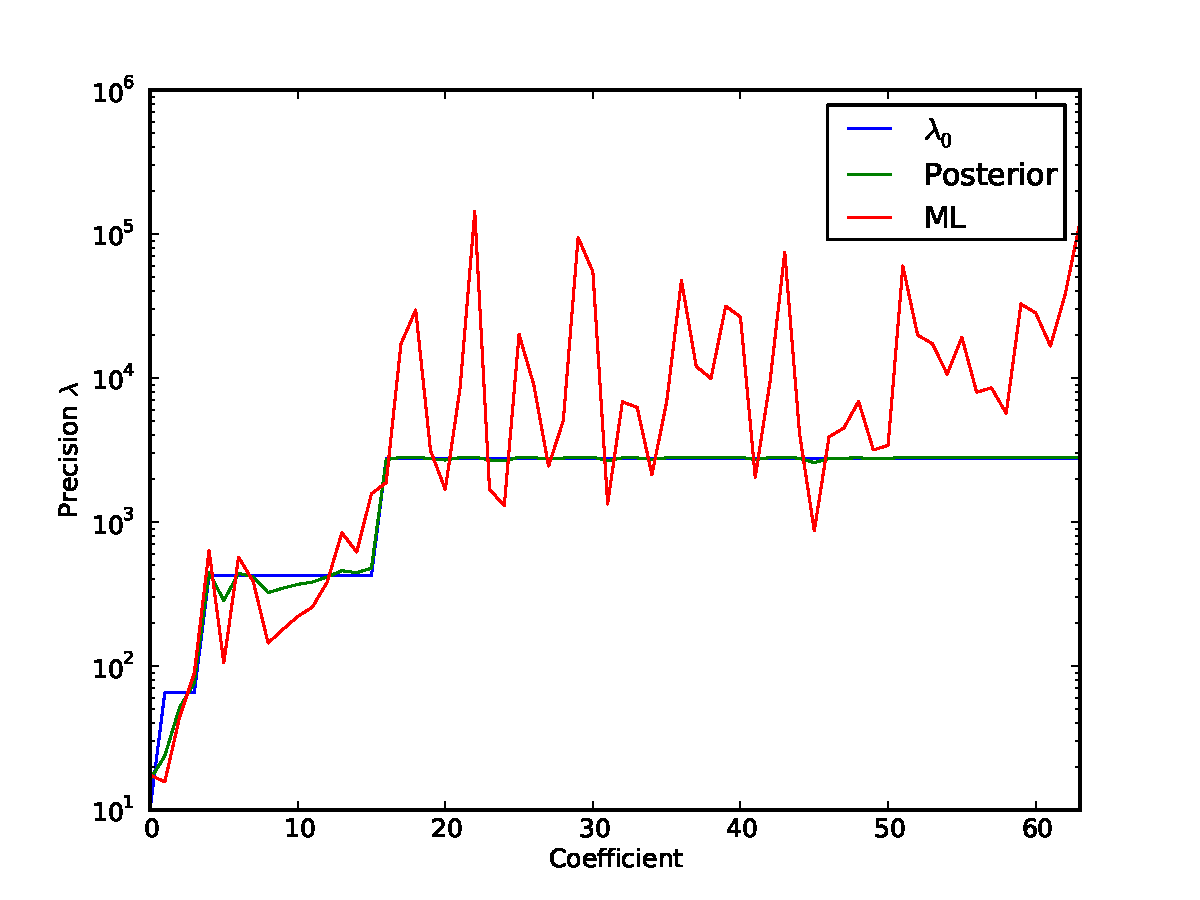
\includegraphics[width=0.8\textwidth]{figs/plotb000-eta10-rho2-7.pdf}
    \caption{Prior ($\lambda_0$), likelihood (ML) and posterior of the coefficients for $\eta=10$ and $\rho=2.7$ at $b_0 = 0.05$. For digit 0, mixture component 0 and axis 0.} \label{fig:rho27}
\end{figure}


\subsection{Iterative training of $\mu$ and $\lambda$}
Plugging $\mu$ and $\lambda$ back in and training, using several iterations, causes the parameters to diverge (fig.~\ref{fig:itercoefs}). To prevent this, we smooth with a Gamma prior, as described earlier. Using iteratively trained parameters for classification will be referred to as SelDeform+Iter.

The following experiment uses $N=100, M=5, \eta=100, \rho=1, S_0=1, S=3, \delta=0.05, \alpha=1.4$. The iterative process is repeated for 12 iterations, testing with several values of $b_0$. The convergence of the precision for several values of $b_0$ is shown in \cref{fig:iter1,fig:iter2,fig:iter3,fig:iter4}. Notice that in each of these figures, most of the parameters tend to the green line, which is the limit value dictated by our smoothing parameters.

\begin{table}
    \begin{center}
        \begin{tabular}{ | l | l | l | l | l | l | l | l | }
            \hline
            Method & $b_0$ & Miss rate & \FT & \TF & Deformed & \#cont. & F undef. \\
            \hline
            SelDeform & - & 2.90\% & 5.60\% & 1.00\% & 67.40\% & 11.55 & 0.00\% \\
            SelDeform+Iter & 0.0005 & 2.70\% & 5.80\% & 1.00\% & 67.40\% & 11.55 & 0.00\% \\
            SelDeform+Iter & 0.005 & 2.60\% & 5.90\% & 1.00\% & 67.40\% & 11.55 & 0.00\% \\
            SelDeform+Iter & 0.05 & 3.00\% & 5.60\% & 1.10\% & 67.40\% & 11.55 & 0.00\% \\
            SelDeform+Iter & 0.5 & 3.80\% & 4.80\% & 1.10\% & 67.40\% & 11.55 & 0.00\% \\
            \hline
        \end{tabular}
    \end{center}
    \caption{Results of classifying after iteratively training, smoothing with $b_0$.} \label{tab:trialb}
\end{table}

\begin{figure}
    \centering
    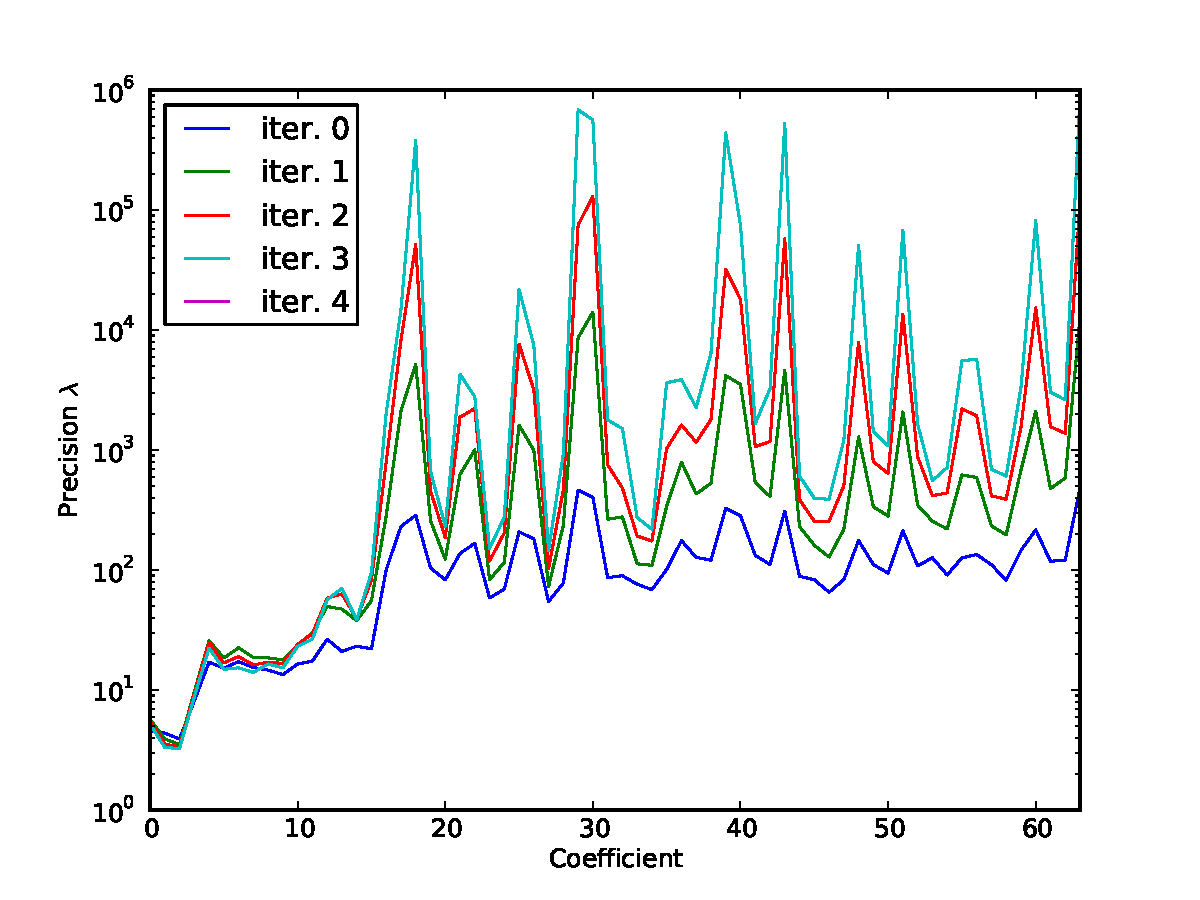
\includegraphics[width=0.8\textwidth]{figs/itercoefs.pdf}
    \caption{Divergence of iteratively training the precision $\lambda$.} \label{fig:itercoefs}
\end{figure}

\begin{figure}
    \centering
    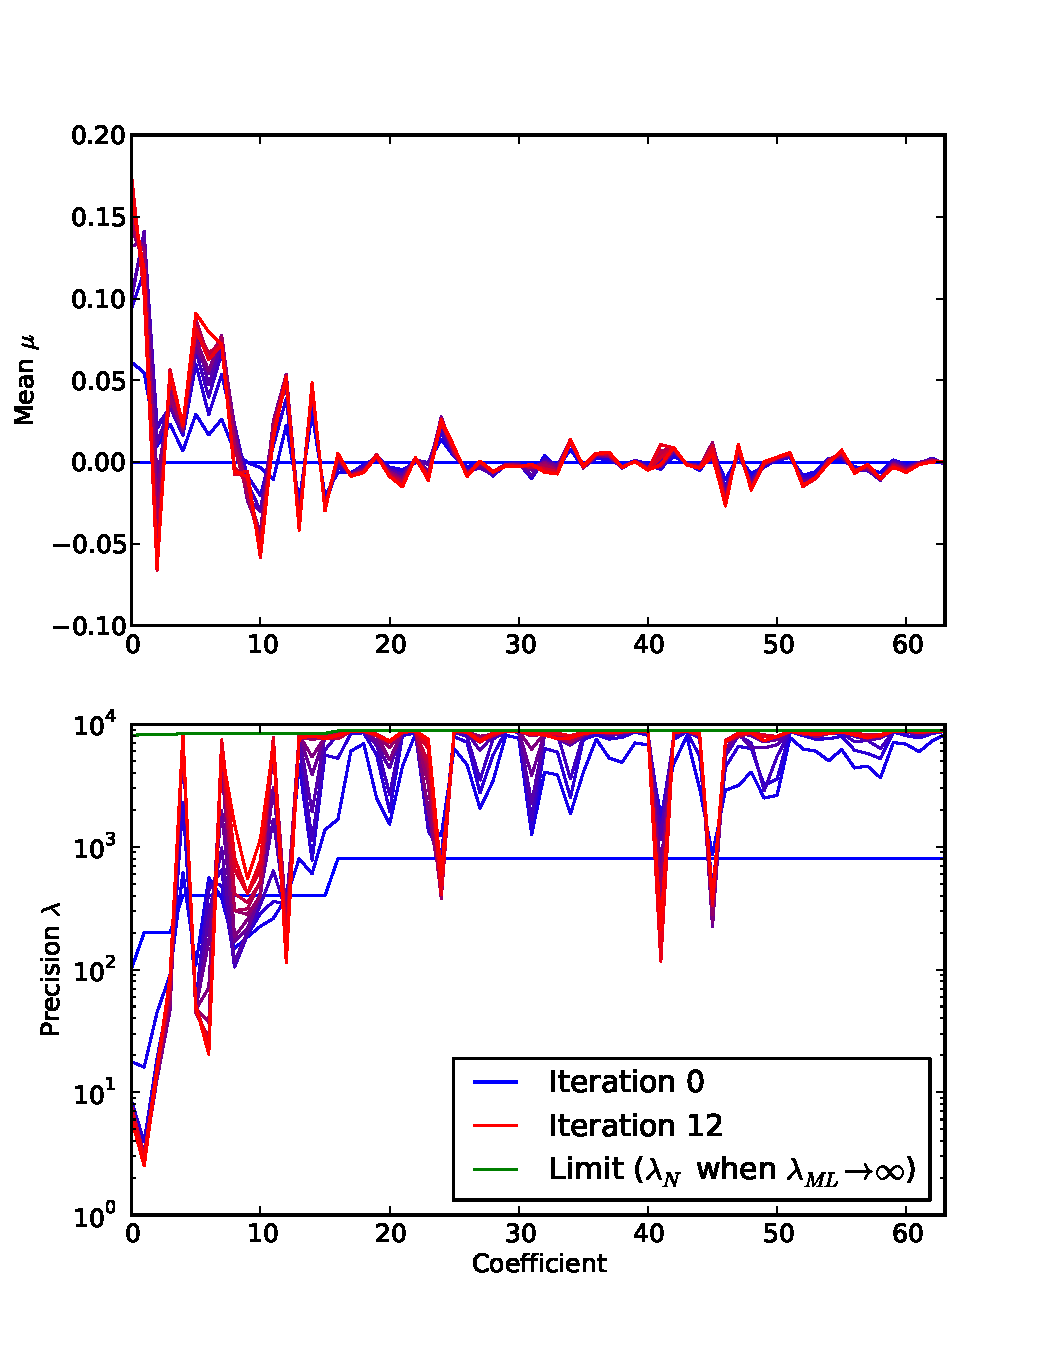
\includegraphics[width=0.8\textwidth]{figs/p1.pdf}
    \caption{Convergence of iteratively training the precision $\lambda$ and smoothing with $b_0 = 0.0005$.} \label{fig:iter1}
\end{figure}

\begin{figure}
    \centering
    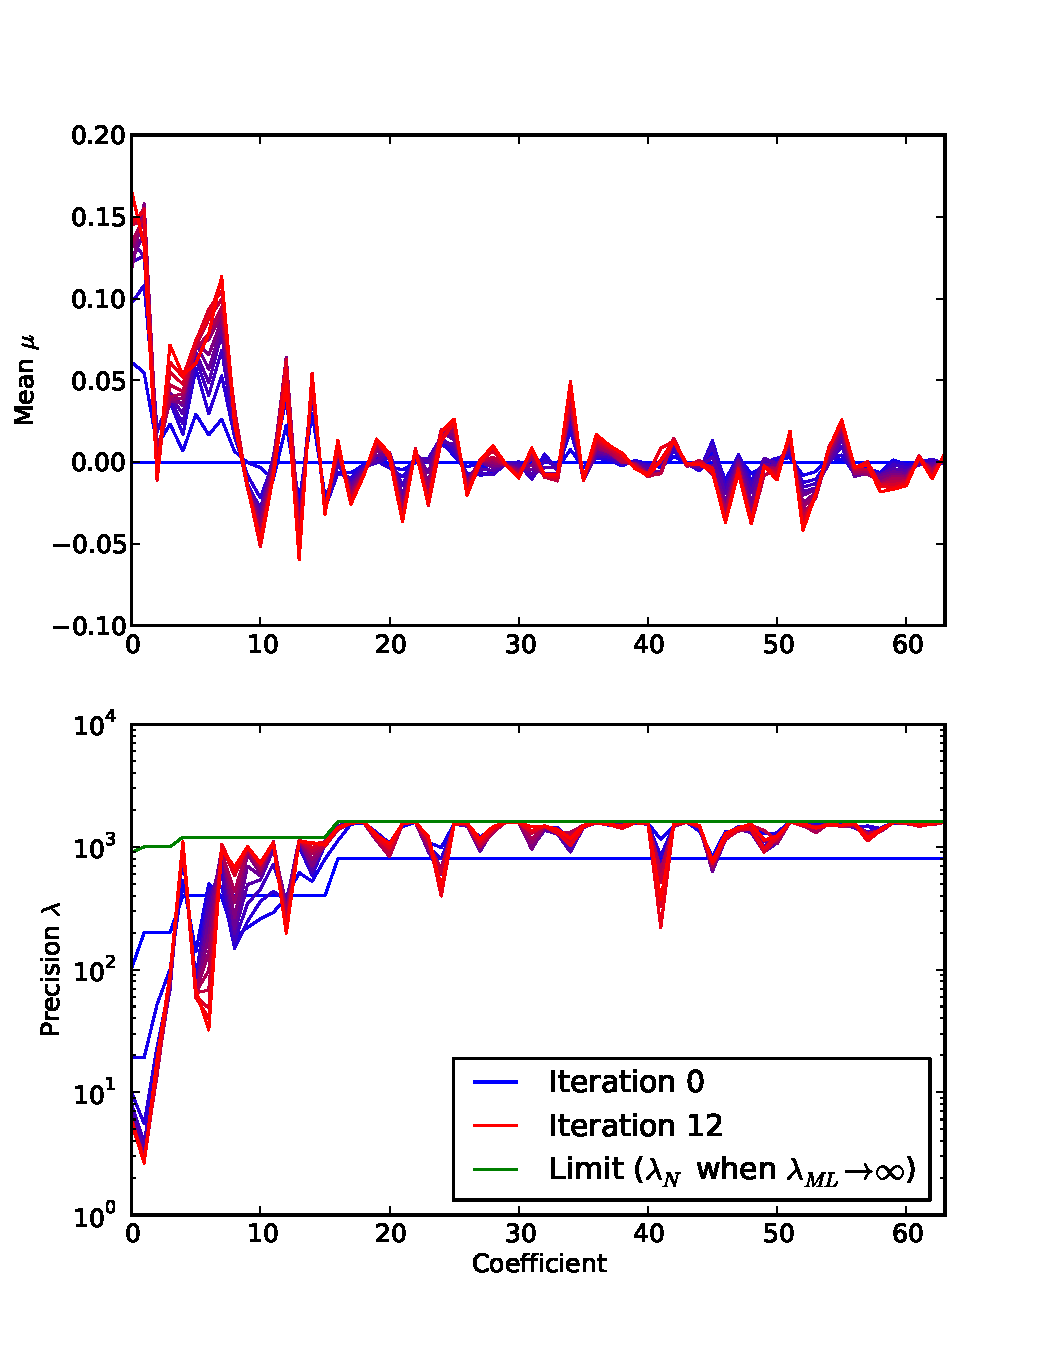
\includegraphics[width=0.8\textwidth]{figs/p2.pdf}
    \caption{Convergence of iteratively training the precision $\lambda$ and smoothing with $b_0 = 0.005$.} \label{fig:iter2}
\end{figure}

\begin{figure}
    \centering
    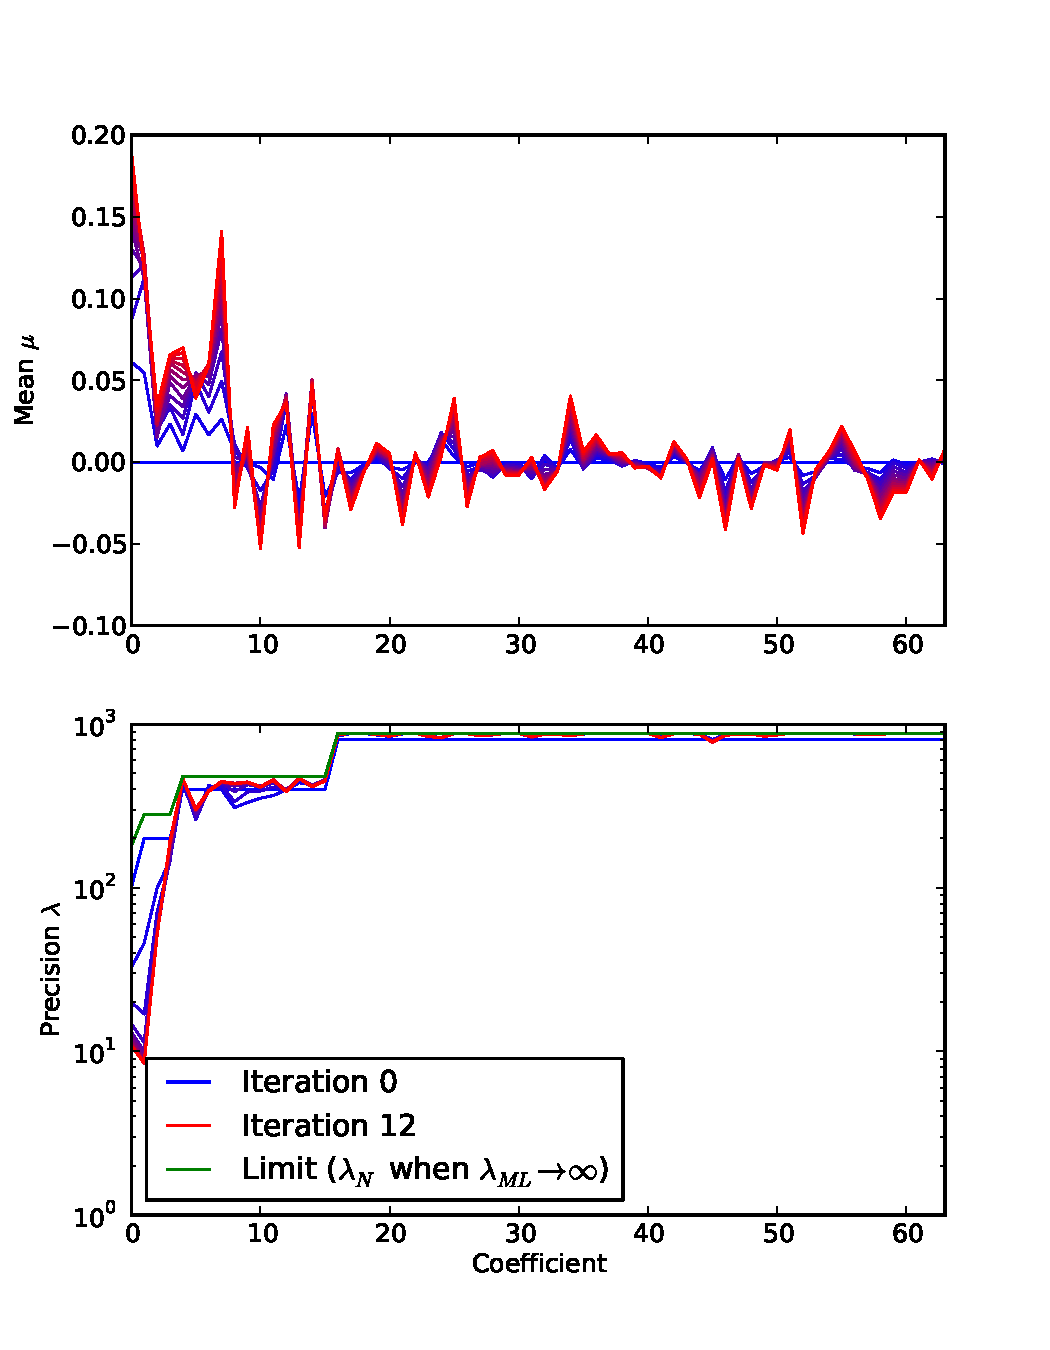
\includegraphics[width=0.8\textwidth]{figs/p3.pdf}
    \caption{Convergence of iteratively training the precision $\lambda$ and smoothing with $b_0 = 0.05$.} \label{fig:iter3}
\end{figure}

\begin{figure}
    \centering
    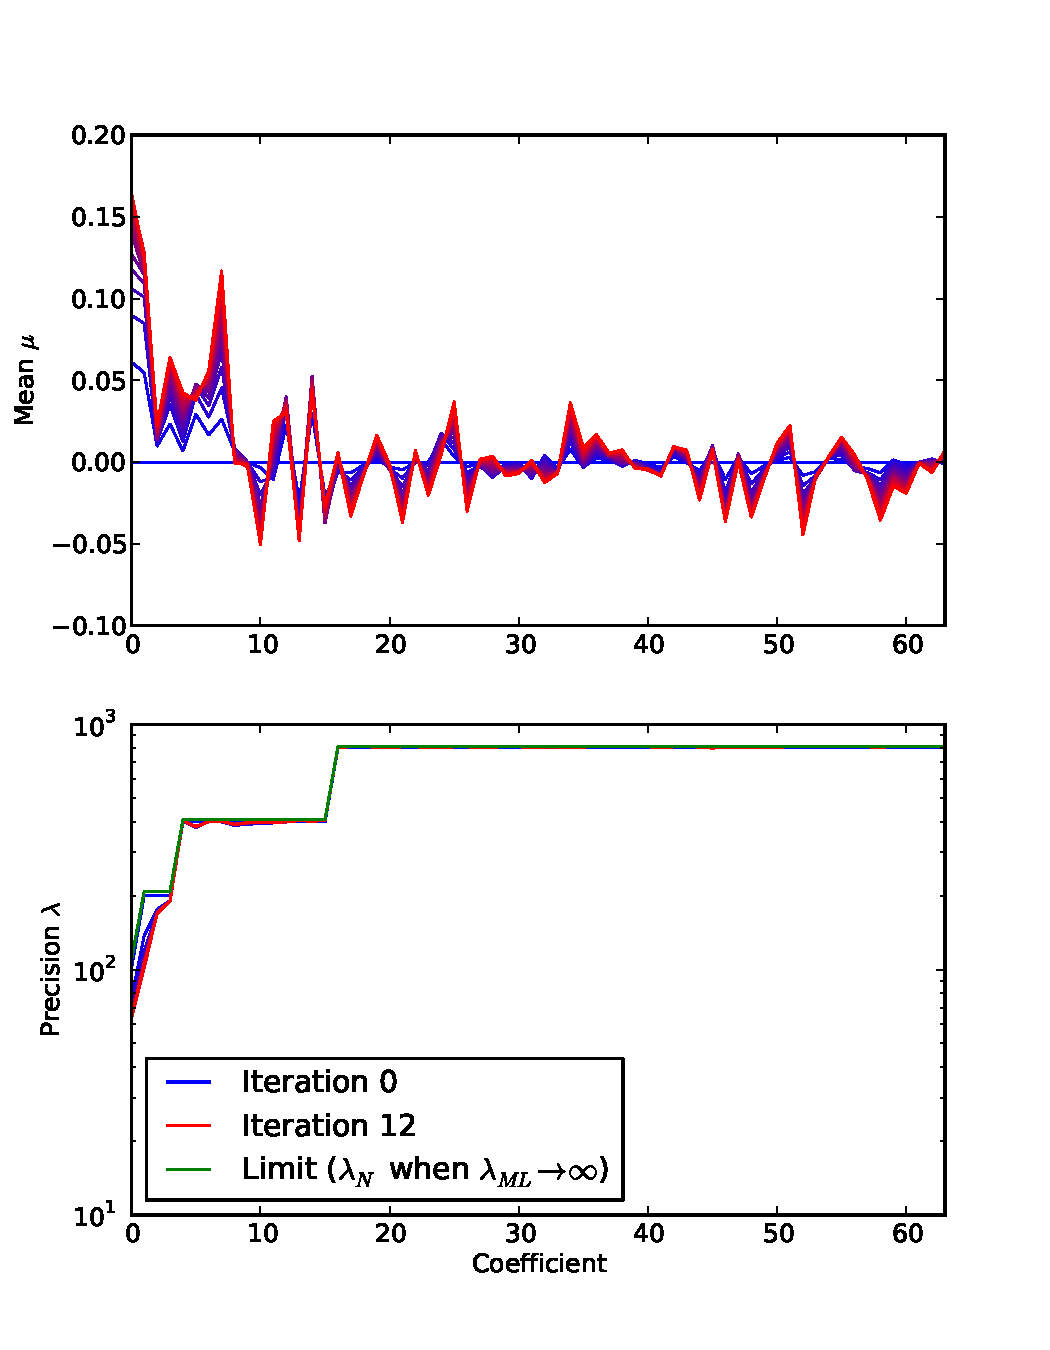
\includegraphics[width=0.8\textwidth]{figs/p4.pdf}
    \caption{Convergence of iteratively training the precision $\lambda$ and smoothing with $b_0 = 0.5$.} \label{fig:iter4}
\end{figure}


\subsection{Observations}
The gradient $\nabla J(u)$ is not $\mathbf{0}$ at the point of convergence in the BFGS algorithm. Exact reason unknown.

\section{Code}
GitHub repositories: \href{https://github.com/gustavla/vision-research/}{gustavla/vision-research}, \href{https://github.com/amitgroup/amitgroup}{amitgroup/amitgroup}

\chapter{Gray-level intensities}

\section{Introduction}
In this chapter, we investigate a data model that uses only gray-level intensities. Most of the training and testing are identical to when we have edge features. The following sections describe the differences.

\subsection{Definitions}

We follow the same definitions as in section \ref{sec:defs}, with the following changes:

\begin{mydef}
Let the family of prototypes be $\mathcal{F} = \{ F \mid F : Z \rightarrow [0, 1]\}$, where the function value represents the intensity value of a pixel.
\end{mydef}

\begin{mydef}
Let the family of images be $\mathcal{I} = \{ I \mid I : L \rightarrow [0, 1]\}$, where the function value represents the intensity value of a pixel. 
\end{mydef}

\section{Data model}
Since we draw the intensities from a normal distribution, we will have both a precision $\lambda$ for the prior, and a precision $\lambda'$ for the likelihood. The latter, $\lambda' \in \mathbb{R}^{|L|}$, is defined for each pixel in the prototype image $F$.
\begin{align}
    u^{(q)}_{k} &\sim \mathcal{N}(\mu^{(q)}_{k}, (\lambda^{(q)}_{k})^{-1}), &q \in Q, k \in K, \label{eq:gaussian} \\
    I(x) &\sim \mathcal{N}(F(\tilde x), (\lambda'_x)^{-1}), &x \in L, j \in J, \label{eq:bernoulli}
\end{align}
The cost and its derivative follow
\begin{align*}
    J(u) =& \frac{1}{2} \sum_{q\in Q} \sum_{k\in K} \lambda^{(q)}_k (u^{(q)}_k -\mu^{(q)}_k)^2 + \frac{1}{2} \sum_{x \in L} \lambda'_x 
            (F(\tilde x) - I(x))^2 
\end{align*}
Taking partial derivatives of this we get
\begin{align*}
    \frac{\partial J(u)}{\partial u^{(q)}_k} =& \lambda^{(q)}_k (u^{(q)}_k -\mu^{(q)}_k) + \sum_{x \in L} 
        \lambda'_x (F(\tilde x) - I(x)) \partial_q F(\tilde x) \psi_k(x).
\end{align*} 


\section{Learning}
In these experiments the prototypes, $F$, were formed by taking the graylevel means of the mixture models computed using edge features. In this way, the method is not entirely built on graylevel intensities.

Training of the parameters is almost identical, expect that now we have $\mu$, $\lambda$ and $\lambda'$. We initialize $\lambda'$ to 1 for each pixel.

Pixels that are background in every sample, will get a 0 variance. To avoid instability, we set the minimum value to $\epsilon$, making the maximum $\lambda'_x$ to $\epsilon^{-1}$. 

\section{Smoothing}
%This time, an increased $\lambda$, will likely result in an increased $\lambda'$. Since both terms will increase, we can see it as a nominal inflation of the cost value, and normalize it (HOW EXACTLY???). This will prevent the values from diverging.
A few attempts of training the parameters iteratively were done, but none with success. We could smooth with a prior as before, although we would need one over both $\lambda$ and $\lambda'$. Since this did not achieve much robustness for edge features, and this would increase the complexity, this was not attempted.

\section{Experiment and results}
Employing a method we will call SelDeform (Intensities) with $N=100, M=5, \eta=100, \rho=1, S_0=1, S=3, \delta=0.05, \alpha=1.4, \epsilon=0.05$. Again, we test on the 1000 samples from the training set, same as before. Results are seen in tab.~\ref{tab:intensity-results}. An example of the parameters are seen in fig.~\ref{fig:intensity-params}.

\begin{figure}
    \centering
    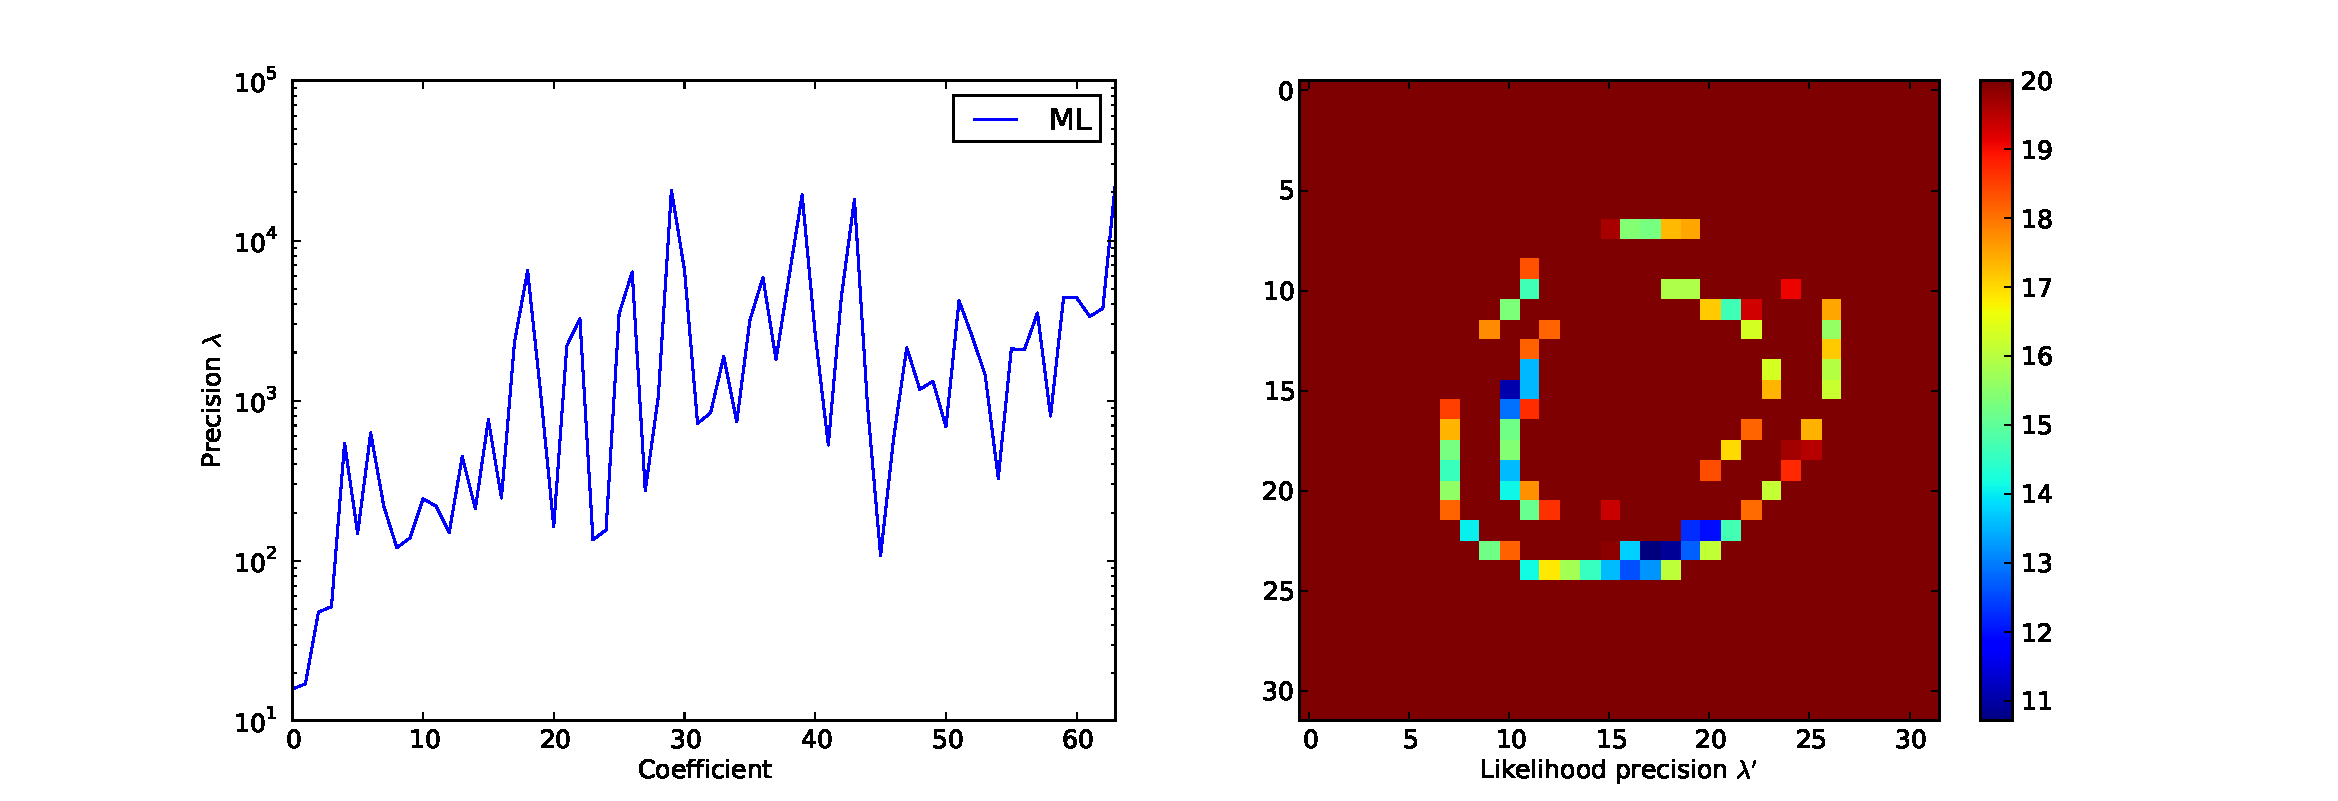
\includegraphics[width=1.0\textwidth]{figs/intensity1.pdf}
    \caption{Intensity parameters after one iteration one trainig. Notice that since $\epsilon=0.05$, we have $\lambda' \le 20$.} \label{fig:intensity-params}
\end{figure}


\begin{table}
    \begin{center}
        \begin{tabular}{ | l | l | l | l | l | l | l | }
            \hline
            Method & Miss rate & \FT & \TF & Deformed & \#cont. & F undef. \\
            \hline
            SelDeform (Intensities) & 4.10\% & 4.40\% & 1.00\% & 67.40\% & 11.55 & 0.00\% \\
            \hline
            SelDeform (Edge-features) & 2.90\% & 5.60\% & 1.00\% & 67.40\% & 11.55 & 0.00\% \\
            \hline
        \end{tabular}
    \end{center}
    \caption{Results for SelDeform (Intensities), compared to its edge-based version.} \label{tab:intensity-results}
\end{table}

\section{Conclusion}
Running the experiments with intensities, as opposed to edge features, gives comparable results (testing set still too small to state enough for sure). Because we set $\epsilon=0.05$, we got a range of $\lambda'$ that spanned less than a factor 2. This suggests that we are likely get similar results if we use a single value for $\lambda'$. However, without $\epsilon$, or with a much smaller $\epsilon$, the precision of the likelihood would change drastically, and so could the results.

\chapter{Feature inflation}

\section{Introduction}
In the first chapter, we inflated the number of edge features, by spreading a feature to its 8 neighbors. If we see this as the result of convolving with a $3\times 3$ inflation kernel of all ones, we can try a few more things. It was implemented by regular convolution and disallowing values to be greater than 1. 

The kernels used are seen in fig.~\ref{fig:kernels}. The kernels "along" are displayed for edges going NE and SW, and are rotated so that they follow {\em along} with the edge.

\section{Experiment and results}
Employing SelDeform+Iter with $N=100, M=5, \eta=100, \rho=1, S_0=1, S=3, \delta=0.05, \alpha=1.4, b_0 = 0.0005$. In all experiments, the specified kernel was used for both training and testing. The experiments were tested on 5000 samples from the training set. The results are seen in tab.~\ref{tab:kernels}.

\begin{table}
    \begin{center}
        \begin{tabular}{ | l | l | l | l | l | l | l | l | }
            \hline
            Kernel & Method & Miss rate & \FT & \TF & Deformed & \#cont. & F undef. \\
            \hline
            box0 & SelDeform+Iter & 9.06\% & 8.68\% & 3.02\% & 99.92\% & 43.87 & 0.00\% \\
            \hline
            box1 & SelDeform+Iter & {\bf 3.10\%} & 6.80\% & 0.94\% & 68.66\% & 12.21 & 0.02\% \\
            \hline
            box2 & SelDeform+Iter & 4.32\% & 6.08\% & 1.48\% & 57.98\% & 9.22 & 0.02\% \\
            \hline
            box3 & SelDeform+Iter & 5.28\% & 6.88\% & 1.74\% & 58.78\% & 8.13 & 0.08\% \\
            \hline
            along1 & SelDeform+Iter & 4.68\% & 8.58\% & 1.50\% & 93.00\% & 27.68 & 0.00\% \\
            \hline
            along2 & SelDeform+Iter & 4.40\% & 8.76\% & 1.46\% & 87.50\% & 21.88 & 0.00\% \\
            \hline
            along3 & SelDeform+Iter & 4.52\% & 8.30\% & 1.36\% & 84.88\% & 19.81 & 0.00\% \\
            \hline
            \hline
            box0 & NoDeform & 14.72\% & - & - & - & - & - \\  
            \hline
            box1 & NoDeform & 8.96\% & - & - & - & - & - \\  
            \hline
            box2 & NoDeform & {\bf 8.92} \% & - & - & - & - & - \\  
            \hline
            box3 & NoDeform & {\bf 8.92} \% & - & - & - & - & - \\  
            \hline
            along1 & NoDeform & 11.76\% & - & - & - & - & - \\  
            \hline
            along2 & NoDeform & 11.70\% & - & - & - & - & - \\  
            \hline 
            along3 & NoDeform & 11.46\% & - & - & - & - & - \\  
            \hline
        \end{tabular}
    \end{center}
    \caption{Results from using different kernels. Top half shows with deformations and bottom half with the mixture model alone.} \label{tab:kernels}
\end{table}

\begin{figure}
    \centering
    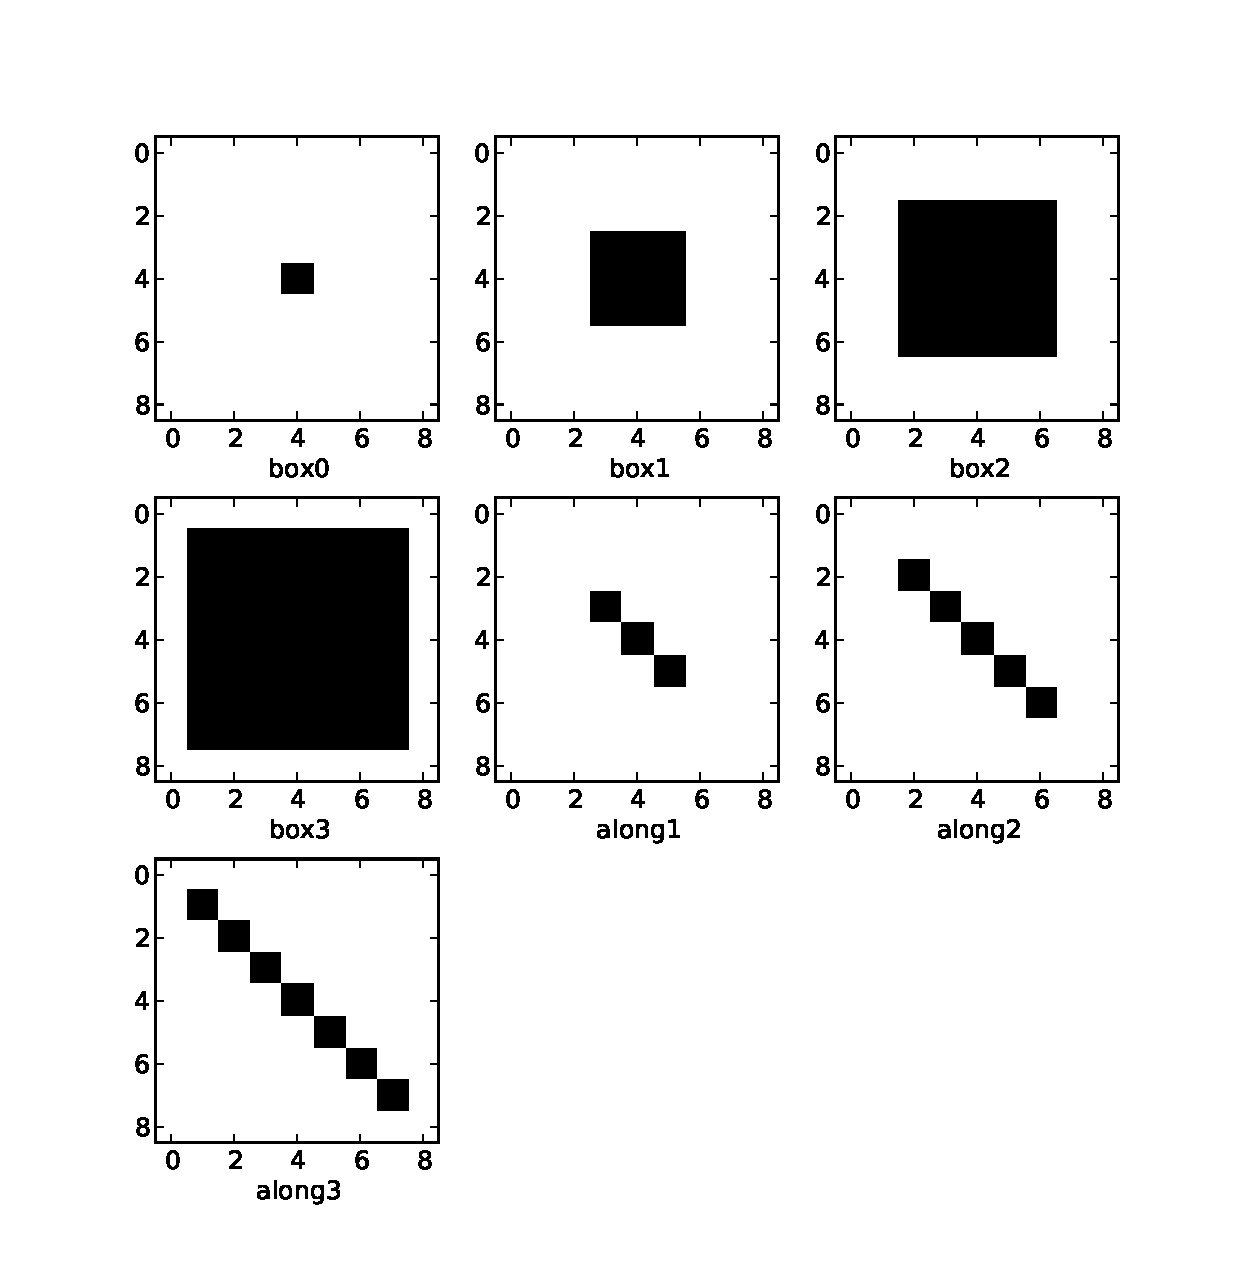
\includegraphics[width=0.8\textwidth]{figs/kernels.pdf}
    \caption{Kernels used to inflate binary edge features with direction NE and SW.} \label{fig:kernels}
\end{figure}


\begin{figure}
        \begin{subfigure}[b]{0.45\textwidth}
                \centering
                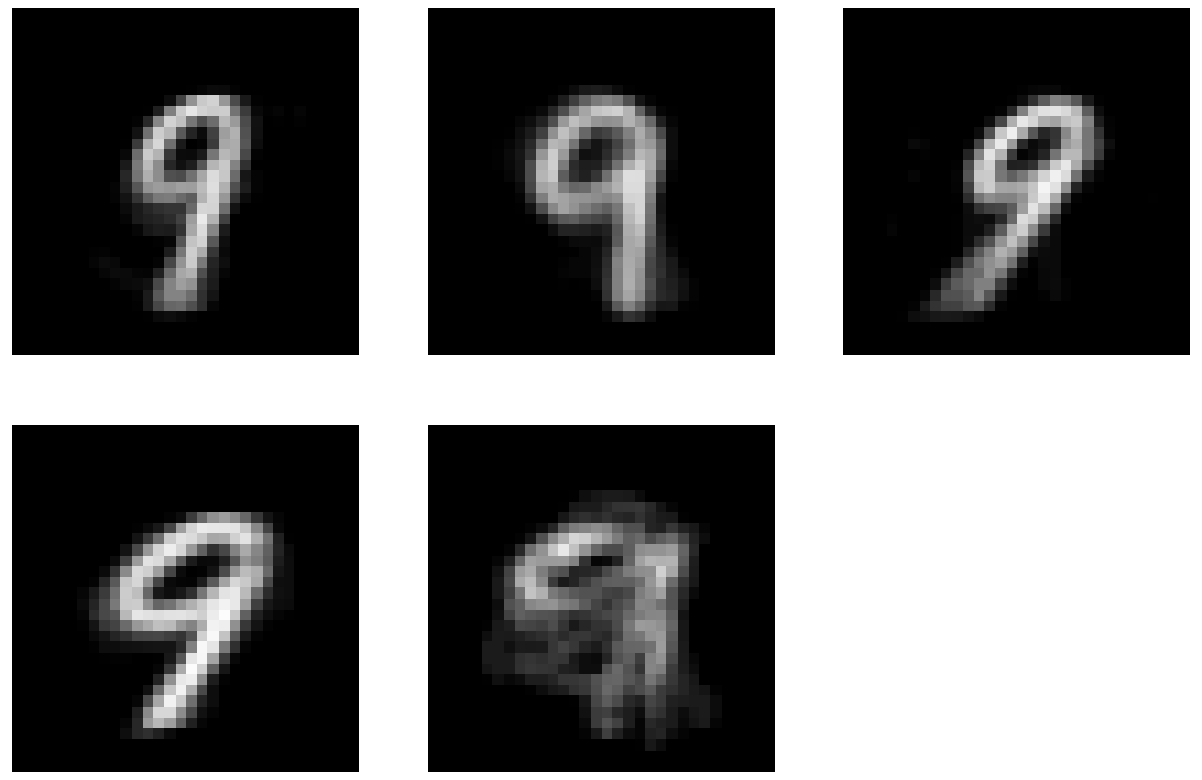
\includegraphics[width=\textwidth]{figs/mixtures9-box1}
                \caption{box1}
                \label{fig:mix9box1}
        \end{subfigure}%
        \qquad %add desired spacing between images, e. g. ~, \quad, \qquad etc. 
          %(or a blank line to force the subfigure onto a new line)
        \begin{subfigure}[b]{0.45\textwidth}
                \centering
                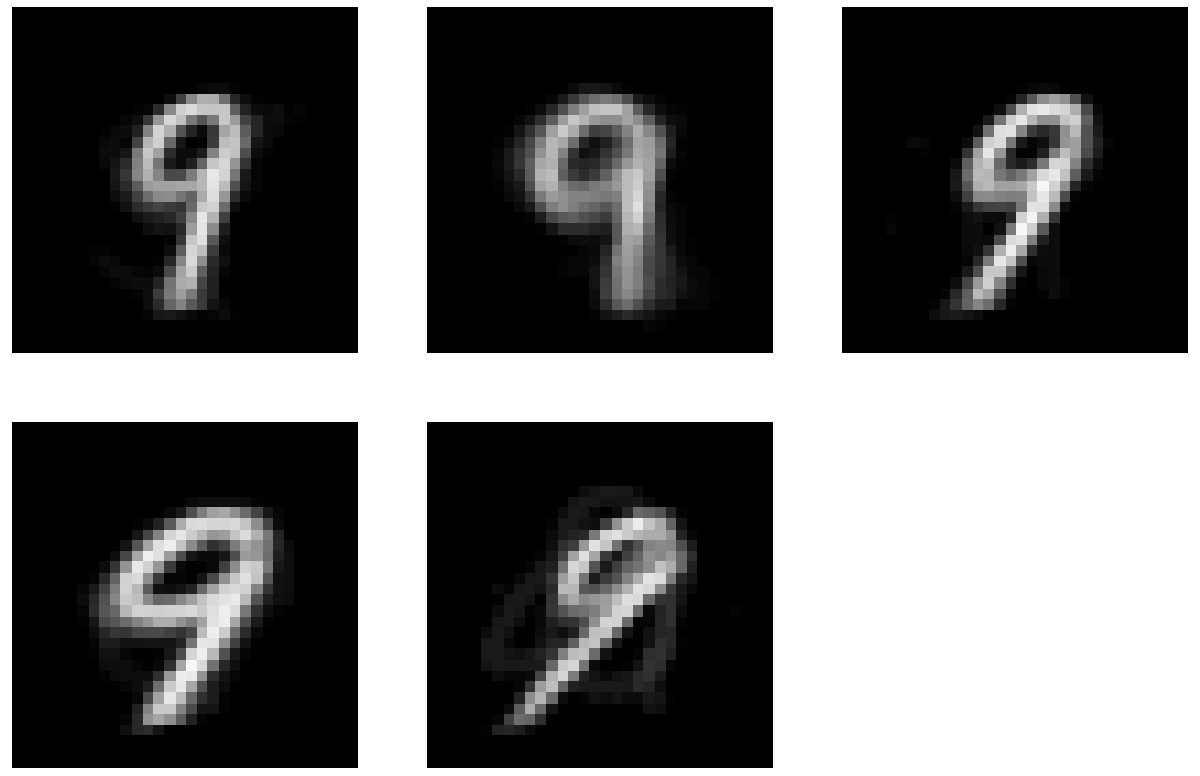
\includegraphics[width=\textwidth]{figs/mixtures9-along1}
                \caption{along1}
                \label{fig:mix9along1}
        \end{subfigure}
        \caption{Gray-level average of mixture components of 9 for two different inflation kernels.}\label{fig:kernelmix}
\end{figure}

\section{Conclusion}
The box1 turned out to give the best results all along. However, it is worth pointing out that the method was built around box1, so some of the parameters of the model could favor this over the other choices.

\end{document}
